\documentclass[10pt,conference]{IEEEtran}
\IEEEoverridecommandlockouts

% \documentclass[acmsmall,screen,review,anonymous]{acmart}
\usepackage{amsmath}
\let\Bbbk\oldBbbk
\usepackage{amssymb}
\usepackage{hyperref}
\usepackage{graphicx}
\usepackage{textcomp}
\usepackage{array}
\usepackage{xcolor}
\usepackage{tcolorbox}
\usepackage{colortbl}
\usepackage{makecell}
\usepackage{svg}
\usepackage[linesnumbered,ruled,vlined]{algorithm2e}
\usepackage{algpseudocode}
\usepackage{multirow}
\usepackage{booktabs}
\usepackage{threeparttable}
\usepackage{enumitem}
\usepackage{caption}
\usepackage{listings}
\usepackage{multicol}
\usepackage{wrapfig}
\usepackage{pdfpages}
\usepackage{tikz}
\usepackage{tabularx}
\newcommand{\mybox}[1]{%
  \begin{tcolorbox}[colback=gray!10,colframe=black,lowerbox=invisible,savelowerto=\jobname_ex.tex,
    left=3pt, right=3pt, top=3pt, bottom=3pt]
    #1
  \end{tcolorbox}
}
\newcommand{\borui}[1]{\noindent\textcolor{purple}{[Borui: {#1}]}}
\newcommand{\afif}[1]{\noindent\textcolor{blue}{[Afif: {#1}]}}
\newcommand{\gias}[1]{\noindent\textcolor{red}{[Gias: {#1}]}}

\begin{document}
\title{Mutation-Guided Hallucination Repair in Large Language Models}
\maketitle

\begin{abstract}
    % Large Language Models (LLMs) frequently produce hallucinations--fluent yet factually incorrect responses--which severely limit their reliability in real-world applications requiring high factual accuracy. Such hallucinations are especially problematic in open-domain question answering and knowledge-intensive scenarios, where users often lack the expertise needed to identify subtle factual errors. While recent studies have proposed various hallucination detection and mitigation techniques, most existing approaches primarily focus on identifying unreliable outputs rather than correcting them. Moreover, many methods rely on external retrieval systems, curated knowledge bases, or additional training or fine-tuning of the underlying models, which introduce practical limitations including restricted availability, domain dependence, privacy concerns, high latency, and poor scalability.


Large Language Models (LLMs) frequently generate hallucinations, which severely limit their reliability in knowledge-intensive tasks and open-domain question answering. Existing detection and mitigation strategies often rely on external retrieval, curated knowledge bases, or resource-heavy fine-tuning, which introduce challenges regarding scalability, latency, privacy, and domain dependency. 
To address these limitations, we propose MutRepair, a hallucination repair framework that uses mutation-guided reasoning and fault-assumption-injected self-correction.
Unlike traditional methods that focus solely on detection or external verification, MutRepair is entirely self-contained and compatible with both open- and closed-source LLMs. The framework operates by systematically generating diverse response mutations (e.g., meaning-preserving rewrites and structural transformation) to expose factual inconsistencies, then guiding the model to repair identified faults through targeted reasoning.
Our evaluation across multiple benchmarks, including knowledge benchmarks and code-reasoning benchmark, demonstrates that MutRepair significantly outperforms state-of-the-art baselines. Across four LLMs (i.e., GPT-4o, GPT-5, Gemini and Qwen3), MutRepair outperforms top baselines by $5.58\% \text{--} 31.58\%$ on average per model (up to $46.68\%$ on individual datasets). These gains are also pronounced on coding tasks, where MutRepair raises the hallucination-repair rate to $6.45\% \text{--} 40.40\%$ . Crucially, MutRepair achieves these improvements while sharply curbing over-correction (i.e., erroneous modification of initially correct answers) by $14.56\% \text{--} 47.59\%$, maintaining high performance stability across multiple runs regardless of model stochasticity.
    
\end{abstract}


\begin{IEEEkeywords}
Large Language Models, Hallucination Repair, Metamorphic Relation, Fault Injection
\end{IEEEkeywords}


\section{Introduction}

Large language models (LLMs), such as the GPT series~\cite{openai2023gpt}, are now embedded as core components of software systems, powering tasks from open-domain question answering to code generation~\cite{huo2024large, champa2024chatgpt, jin2024simllm, lian2024imperfect}. Yet a critical reliability challenge persists: LLMs are prone to \emph{hallucinations} -- outputs that appear fluent and coherent yet are factually incorrect or unfaithful to ground truth~\cite{ji2023survey, xu2024hallucination}. Figure~\ref{fig:haluexample} illustrates such a natural-language hallucination from ChatGPT in the legal domain, where the model confidently asserts false information that could mislead users and erode trust in production deployments. Crucially, hallucinations are not confined to natural language: when an LLM generates code, the same failure surfaces as non-existent API calls, incorrect boundary conditions, or flawed logic that silently break the program\cite{tian2025codehalu}. From a software engineering perspective, both forms constitute a single class of defect -- a knowledge-intensive component emitting plausible but incorrect artifacts~\cite{fan2023llmse, zhou2025lost, zhang2023siren} -- placing hallucination squarely among classic SE concerns such as test oracle construction, automated testing, and automated program repair.

A growing body of work investigates hallucination detection~\cite{huo2023retrieving, lewis2020retrieval, yao2023llm, wu2025detecting}, yet detection alone is insufficient: users and downstream systems require reliable artifacts, not merely warnings. This necessitates hallucination repair -- actively correcting erroneous outputs into faithful ones. Existing repair approaches typically fine-tune the model~\cite{kumar2025training} or ground outputs through retrieval-augmented generation (RAG)~\cite{ayala2024reducing}, but both depend on external resources -- knowledge bases, auxiliary models, or retraining pipelines -- that are inaccessible for black-box LLMs and unavailable in specialized or emerging domains. This motivates a lightweight, inference-time repair framework that requires no such resources, which in turn raises the test oracle problem: at repair time no ground truth is available, so the system must judge correctness from the model's own outputs alone. This is what makes repair fundamentally harder than detection, and it also demands avoiding over-correction -- the analogue of a regression-inducing patch in automated program repair~\cite{petke2024patch} -- since corrupting an originally correct output is as harmful as leaving a hallucination unrepaired.

\begin{figure}[htbp]
    \centering
    
\includegraphics[width=0.8\linewidth]{figures/haluexample.pdf}
    \caption{An example of a hallucination output generated by ChatGPT in legal domain.}
    \label{fig:haluexample}
\end{figure}

In this paper, we present MutRepair, a hallucination repair framework that recasts hallucination as a repairable fault and adapts metamorphic relations, fault injection, and automated repair to LLM outputs. Our key insight is that a single output offers no leverage for self-assessment, whereas a family of controlled variants does: by transforming the base response under metamorphic relations, MutRepair expands one answer into a diverse repair space in which faults surface through cross-variant comparison. MutRepair operates in three stages. \emph{(1) Mutation Construction} generates MR-guided mutations of the base response to expose latent faults. \emph{(2) Fault-Injected Self-Repair} injects an explicit fault assumption into each mutation, shifting the model from passive validation into active fault localization and repair. \emph{(3) Aggregation} selects the final patch through a self-contained comparative oracle that ranks the independently repaired candidates against one another, requiring no external ground truth. The same framework instantiates on both natural language and code, differing only in its modality-specific mutation operators, demonstrating that the paradigm is not specific to natural language but a general, SE-grounded mechanism for repairing faults in LLM-generated artifacts.

We conduct an extensive empirical evaluation across two modalities: three natural-language hallucination benchmarks -- TruthfulQA~\cite{lin2022truthfulqa}, HotpotQA~\cite{yang2018hotpotqa}, and FreshQA~\cite{vu2023freshllms} -- and a code-generation benchmark built from LeetCode problems, spanning four representative LLMs (GPT-4o, GPT-5, Gemini, and Qwen3). We compare MutRepair against strong self-contained baselines (CoT~\cite{wei2022chain}, CoVe~\cite{dhuliawala2024chain}), a retrieval-augmented variant (CoVe-SE), and DrHall~\cite{wu2025detecting}, a state-of-the-art metamorphic-testing-based method from the SE community. Across all settings, MutRepair consistently outperforms every baseline: it improves hallucination repair by $5.58\%\text{--}31.58\%$ on average per model on natural-language tasks (up to $46.68\%$ on individual datasets) and raises the repair rate by $6.45\%\text{--}40.40\%$ on code, while sharply curbing over-correction by $14.56\%\text{--}47.59\%$ relative to the strongest baseline. It further exhibits strong run-to-run robustness and remains stable under varying temperature and mutation configurations.

Our major contributions include:
\begin{enumerate}[leftmargin=20pt]
    \item We reframe LLM hallucination as a repairable fault and propose MutRepair, to the best of our knowledge the first framework to adapt metamorphic mutation, fault-assumption injection, and automated repair into a unified, self-contained hallucination repair pipeline that requires no external knowledge, auxiliary models, or ground-truth feedback.
    \item We design relation-guided mutation operators and a comparative aggregation stage, and show that the same pipeline instantiates across modalities -- differing only in its modality-specific mutation operators -- demonstrating that mutation-guided repair generalizes beyond natural language to code-generation faults.
    \item We conduct a comprehensive study on three natural-language benchmarks and a code benchmark across four LLM families, comparing against self-contained, retrieval-augmented, and SE-based baselines, and show that MutRepair consistently achieves higher repair effectiveness with substantially lower over-correction.
\end{enumerate}

\begin{figure*}[t]
    \centering
    
\includegraphics[width=1\textwidth]{figures/workflow.pdf}
    \caption{General workflow of MutRepair}
    \label{fig:workflow}
\end{figure*}

\section{Methodology}
MutRepair is a self-contained hallucination repair framework that treats a hallucinated LLM output as a repairable fault, and corrects it without any external knowledge or ground-truth feedback. Given a question and its base response $B$ from the LLM, MutRepair repairs $B$ through three stages (see Figure~\ref{fig:workflow}):
\textit{(1) Mutation Construction}, which expands $B$ into a set of relation-guided variants using metamorphic relations to expose latent faults;
\textit{(2) Fault-Injected Self-Repair}, which treats each variant as potentially faulty and prompts the model to actively re-examine and repair it under an explicit fault assumption; and
\textit{(3) LLM-as-Judge Aggregation}, which compares the independently repaired candidates against one another and selects the most reliable one as the final answer.
The framework is modality-agnostic: the same three stages apply to both natural language and code, differing only in the mutation operators of Stage~1, while the fault-injected repair and comparative aggregation stages -- neither of which relies on an external oracle -- are shared across modalities. Algorithm~\ref{alg:mt-repair-ranking} presents the complete procedure, from the initial response to the selection of the final repaired answer.

\begin{algorithm}
\caption{MutRepair: Mutation-Guided Hallucination Repair}
\label{alg:mt-repair-ranking}
\small
\KwIn{
    Question $Q$, 
    Base Response $B$,
    Mutation Prompt $P_m$, 
    Verification Prompt $P_a$, 
    Ranking Prompt $P_r$
}
\KwOut{
    Repaired Answer $A^*$
}
\SetKwFunction{LLM}{LLM}
\SetKwProg{Fn}{Function}{:}{}
\SetAlgoNlRelativeSize{0}
\setcounter{AlgoLine}{0}
\Fn{\textbf{Repair}}{
    \textbf{// Stage 1: Mutation Construction} \\
    $M \gets \LLM(Q, B, P_m)$
    
    $M \gets M \cup \{B\}$
    
    \textbf{// Stage 2: Fault-Injected Self-Repair} \\
    $A \gets \emptyset$
    
    \ForEach{$m \in M$}{
        $a_m \gets \LLM(Q, m, P_a)$
        
        $A \gets A \cup \{a_m\}$
    }
    
    \textbf{// Stage 3: LLM-as-Judge Aggregation} \\
    $n \gets |A|$
    
    Initialize ranking matrix $R \in \mathbb{N}^{n \times n}$
    
    \For{$i \gets 1$ \KwTo $n$}{
        \For{$j \gets 1$ \KwTo $n$}{
            $R_{i,j} \gets \LLM(a_i, a_j, Q, P_r)$
            
            Given score \([1,n]\)
        }
    }
    \For{$i \gets 1$ \KwTo $n$}{
        $S(a_i) \gets \sum_{j=1}^{n} R_{i,j}$ 
    }
    $A^* \gets \arg\min_{a_i \in A} S(a_i)$ 
    
    \KwRet{$A^*$}
}
\end{algorithm}

\subsection{Mutation Construction}
This stage is illustrated in Algorithm~\ref{alg:mt-repair-ranking} (lines~2--4). Given a question $Q$ and its base response $B$, MutRepair treats $B$ as a candidate artifact under test and systematically perturbs it into a set of structured variants $M = \{m_1, m_2, \dots, m_k\}$ (line~2), where each $m \in M$ is a metamorphic follow-up derived from $B$. Rather than repeatedly regenerating an answer to the same prompt, these variants place $B$ under controlled, semantics-related transformations, so that latent factual or logical errors surface as inconsistencies across the variant set.

Metamorphic relations (MRs), originating from metamorphic testing in software engineering, characterize how a system's outputs are expected to change or remain invariant under controlled transformations of related inputs, without requiring an explicit oracle~\cite{chen2018metamorphic, zhang2014search, cho2025metamorphic}. We instantiate three modality-agnostic relations that apply to both natural-language answers and generated code. For a natural-language response, we represent $B$ as a relational statement $B = \langle sub, verb, obj \rangle$, where $sub$ and $obj$ denote the subject and object entities and $verb$ captures the core predicate; an analogous decomposition applies to a code statement at the level of its operations and operands. The three relations are defined as structured transformations from $B$ to $m$:

\begin{equation}
    \langle sub, verb_{1}, obj \rangle \Rightarrow m = \langle sub, verb_{2}, obj \rangle
\end{equation}
\noindent\textbf{(1) Meaning-Preserving Rewrite}, where $verb_{2}$ is semantically close to $verb_{1}$ but realized in a different surface form, preserving the asserted content.

\begin{equation}
    \langle sub, verb, obj \rangle \Rightarrow m = \langle obj, verb', sub \rangle
\end{equation}
\noindent\textbf{(2) Structural Transformation}, where $verb'$ is adapted so that the statement is restructured (e.g., subject--object reordering or active--passive inversion) without altering its meaning.

\begin{equation}
    \langle sub, verb, obj \rangle \Rightarrow m = \langle sub, \neg verb, obj \rangle
\end{equation}
\noindent\textbf{(3) Semantic Polarity Shift}, where $\neg verb$ denotes a targeted inversion (e.g., an antonym, negation, or an added or removed condition) that probes hidden assumptions in $B$.

These three relations capture the lexical, structural, and semantic dimensions along which a response can be perturbed, and apply uniformly across modalities. Code, however, is a structured artifact whose fault space extends beyond surface form to algorithmic and data-structural choices. Specifically, for code we introduce a fourth, modality-specific operator: \textbf{(4) Algorithm/Data-Structure Variant}, which replaces the core algorithm or data structure of $B$ with a equivalent alternative (e.g., recursion to iteration or memoization to tabulation), exposing faults that are invisible to purely surface-level rewrites. Figure~\ref{fig:codemut} illustrates this operator on a representative code mutation.

At the end of this stage, in addition to the generated variants, the original base response $B$ is also added to $M$ (line~4), ensuring that both the initial and mutated answers are carried into the subsequent self-repair process. The prompt template below illustrates mutation generation for a natural-language response; the prompt for code follows the same structure, additionally invoking the algorithm/data-structure operator and requiring each mutation to remain a complete, runnable program.

\begin{tcolorbox}[
    colback=green!6,
    colframe=green!40!black,
    title=Metamorphic mutations Generation,
    fonttitle=\bfseries,
    fontupper=\small,
    boxrule=0.6pt,
    arc=2pt,
    left=2pt,
    right=2pt,
    top=2pt,
    bottom=2pt
]
\textbf{Instruction:} Generate mutations of the base response base on the origin question.

\vspace{2pt}
\textbf{QA pair:} Question: On what date was the Declaration of Independence officially signed?

Answer: The Declaration of Independence was officially signed on August 2, 1776.

\vspace{2pt}

\textbf{Prompt:} Given a question and its base response, generate $n$ diverse single-sentence mutations of the response, applying each of the following metamorphic relations at least once:\\
1. ~\emph{Meaning-Preserving Rewrite}\\
2. ~\emph{Structural Transformation}\\
3. ~\emph{Semantic Polarity Shift} \ldots

\vspace{2pt}
\textbf{Mutations:}
1. The official signing date of the Declaration of Independence was August 2, 1776.

2. On August 2, 1776, the Declaration of Independence was formally signed. \ldots
\end{tcolorbox}

\subsection{Fault-Injected Self-Repair}

Given the variant set $M$, MutRepair repairs the potential fault carried by each variant and produces a set of repaired candidates $A$ (Algorithm~\ref{alg:mt-repair-ranking}, lines~5--9). This stage adapts two complementary paradigms from software reliability engineering: fault injection, which deliberately assumes a fault to expose latent weaknesses, and automated program repair, which synthesizes a correction under that assumption rather than merely flagging the defect. We adopt the core idea -- not the testing machinery -- of fault injection: by explicitly assuming that a response is faulty, we drive the model to localize and repair the error instead of passively validating it.

This design targets a well-documented obstacle: LLMs exhibit confirmation bias when re-examining their own outputs, tending to confirm ~\cite{yu2025survey} rather than critically assess them ~\cite{pan2023automatically}. Simply re-prompting the model to ``check'' a response therefore rarely surfaces its own errors. Instead, we treat each variant $m \in M$ as a potentially faulty instance and inject an explicit fault assumption into the prompt (line~7--8): the model is told that the response may contain an error -- a factual mistake for a natural-language answer, or faulty logic, a non-existent API, or a boundary error for code -- and is required to re-examine it, preserve it if no error is found, and otherwise produce a corrected version. This assumption shifts the model from a passive validation mode into an active fault-localization-and-repair mode, eliciting the deeper self-scrutiny that plain regeneration or rephrasing does not.

The same fault-injection prompt is applied uniformly to both natural-language and code variants, requiring no modality-specific adaptation. Repairing all variants independently yields a set of repaired candidates $A$ (line~9), which are passed to the LLM-as-judge aggregation stage. The prompt template is shown below.

\begin{tcolorbox}[
    colback=green!6,
    colframe=green!40!black,
    title=Fault-injected Self-repair Prompt,
    fonttitle=\bfseries,
    fontupper=\small,
    boxrule=0.6pt,
    arc=2pt,
    left=2pt,
    right=2pt,
    top=2pt,
    bottom=2pt
]
\textbf{Instruction:} Assume the response may be faulty; re-examine it and repair any error.

\vspace{2pt}
\textbf{Prompt: The response below may contain hallucination.} Verify it step by step and return a single corrected, faithful answer. If it is already correct, return it unchanged; otherwise, produce the corrected version. Do not introduce unsupported details or non-existent references. ...
\end{tcolorbox}


\subsection{LLM-as-Judge Aggregation}\label{sec:llmasjudge}
After fault-injected self-repair, MutRepair obtains a set of independently repaired candidates $A$, each derived from a different variant of the base response (Algorithm~\ref{alg:mt-repair-ranking}, lines~10--20). These candidates may still differ in correctness and quality, so the final stage performs LLM-as-judge aggregation to evaluate them and select the most reliable answer. This step is analogous to test oracle construction and patch validation in software engineering, where multiple candidate fixes are assessed and only the most plausible one is accepted; it is motivated by recent studies~\cite{li2025generation, zeng2024llm} showing that LLMs can act as effective judges for answer evaluation without relying on external resources.

We adopt a pairwise ranking strategy to aggregate the repaired candidates. Rather than scoring each candidate in isolation or producing an absolute confidence score, MutRepair compares the candidates against one another, with each comparison yielding a \emph{relative} score that reflects the two candidates' comparative quality with respect to the original question. Aggregating these relative scores across all comparisons induces an overall ranking, from which the best-ranked candidate is selected as the final answer. This relative formulation is more reliable than absolute scoring, as comparing two answers is an easier judgment for an LLM than calibrating the correctness of a single one, and it directly alleviates the selection bottleneck in hallucination repair. We quantify the resulting computational cost in Section~\ref{sec:6.1}.

Concretely (lines~11--16), MutRepair populates a score matrix $R$ over the candidate set $A$: for each pair $a_i$ and $a_j$ (line~15), it feeds the original question $Q$ and the two candidates to the LLM under a fixed judging-criteria prompt, and the LLM returns a score in $[1, n]$ (line~16), where a lower score marks the candidate that better answers the question. The total score of each candidate is then obtained by summing its row in $R$ (lines~17--18), and the candidate with the lowest total score is returned as the final output $A^*$ (lines~19--20). Like the preceding stages, this aggregation is self-contained and applies identically across modalities. The prompt template of this stage is shown below.

\begin{tcolorbox}[
    colback=green!6,
    colframe=green!40!black,
    title=Pairwise Ranking Prompt,
    fonttitle=\bfseries,
    fontupper=\small,
    boxrule=0.6pt,
    arc=2pt,
    left=2pt,
    right=2pt,
    top=2pt,
    bottom=2pt
]
\textbf{Instruction:} Compare the candidate answers pairwise and score each one to support final selection.

\vspace{2pt}
\textbf{Prompt:} You are given a question and $n$ candidate answers. Examine each candidate in the context of the question and assign it a score in $[1, n]$ reflecting its factual soundness and how well it answers the question, where a lower score indicates a better answer. Assess each candidate relative to the others, and return only the scores. ...
\end{tcolorbox}


\section{Experimental Setup}
\subsection{Research Questions}
We formulate the following research questions (RQs) to systematically evaluate the effectiveness, internal mechanisms, and robustness of MutRepair:
\begin{enumerate}[leftmargin=30pt, label=\textbf{RQ\arabic{*}.}]
    \item \textbf{Effectiveness and Generalization:} How effectively does MutRepair repair hallucinations across both natural-language and code generation tasks, compared to baselines?
    \item \textbf{Component Analysis:} How do the key components of MutRepair contribute to its hallucination repair performance?
    \item \textbf{Stability and Robustness:} How robust is MutRepair to LLM stochasticity, and how sensitive is it to key parameters such as temperature and the number of mutations?
\end{enumerate}
RQ1 evaluates whether MutRepair can effectively repair hallucinations and outperform state-of-the-art baselines, while simultaneously controlling the risk of over-correction.  
RQ2 investigates the internal mechanisms of MutRepair by analyzing the effects of different aggregation strategies and isolating the contributions of mutation-guided repair, as well as characterizing the remaining upper-bound repair potential.  
RQ3 examines the stability and robustness of MutRepair under repeated runs and studies its sensitivity to key generation parameters, in order to understand how stochasticity and parameter choices influence repair effectiveness and safety.


\subsection{Baselines}
We compare MutRepair against state-of-the-art self-contained baselines that require no additional training, organized into three methods: \textbf{Chain-of-Thought (CoT)}~\cite{wei2022chain}, \textbf{Chain-of-Verification (CoVe)}~\cite{dhuliawala2024chain}, and \textbf{DrHall}~\cite{wu2025detecting}. Together they cover complementary repair strategies -- internal reasoning, self-verification, and metamorphic-relation-guided repair. CoT and DrHall apply to both natural-language and code generation tasks, whereas CoVe is designed for natural language.

\paragraph{Self-contained baselines}
\textbf{Chain-of-Thought} prompting instructs the LLM to reason through a problem step by step before producing its final answer. It is a standard baseline for eliciting the latent reasoning ability of modern LLMs, and applies directly to both natural-language answers and generated code. \textbf{Chain-of-Verification} prompts the LLM to extract key entities or factual claims from an initial response, generate verification questions about them, answer those questions using the LLM itself, and inject the verification results back to reassess and revise the original answer; we apply it to natural-language tasks. \textbf{DrHall}~\cite{wu2025detecting} is a recent software-engineering method that, like MutRepair, leverages metamorphic testing to repair hallucinations, and likewise applies to both natural-language and code tasks. The key distinction is where the metamorphic transformation is applied: DrHall constructs variants of the input question and checks the model's answers for consistency across them. Among the variants reported in the DrHall paper, we adopt its best-performing configuration that requires no external knowledge, ensuring a fair comparison under our self-contained setting.

\paragraph{Non self-contained baseline}
\textbf{Chain-of-Verification with Search Engine (CoVe-SE)} is a variant of CoVe that answers the generated verification questions using a search engine rather than the LLM itself. Although it is no longer self-contained, CoVe-SE serves as a representative retrieval-augmented (RAG-style) baseline, enabling comparison between MutRepair and approaches that rely on external knowledge sources.

We note that several recent methods extend the verification idea beyond CoVe~\cite{wu2024large, song2025progco, he2024retrieving}. We do not adopt them as primary baselines because they rely on external program execution or are designed for closed-form selection (e.g., multiple-choice) and mathematical reasoning tasks.


\subsection{Datasets}
We evaluate MutRepair across two modalities. For natural language, we adopt three widely used benchmarks that cover complementary hallucination scenarios: TruthfulQA~\cite{lin2022truthfulqa} for misconception- and bias-driven hallucinations, HotpotQA~\cite{yang2018hotpotqa} for reasoning-induced hallucinations, and FreshQA~\cite{vu2023freshllms} for timeliness-related hallucinations. For code, we adopt LeetCodeDataset~\cite{xia2025leetcodedataset} to assess whether the same framework generalizes to code-generation hallucinations.

\subsubsection{TruthfulQA}
We use the full set of 817 questions across 38 categories (e.g., health, law, finance), which are designed to elicit responses influenced by widespread misconceptions and false beliefs.

\subsubsection{HotpotQA}
HotpotQA poses multi-hop questions that require reasoning over multiple supporting facts. From its 113K questions, we randomly sample 610; following statistical sampling theory with finite population correction, this yields a 99\% confidence level at a 5\% margin of error under $p=0.5$.

\subsubsection{FreshQA}
FreshQA targets hallucinations arising from outdated or missing knowledge. To ensure fair evaluation across model training cutoffs, we retain 399 questions whose answers were established before 2024 and remain stable over time, excluding rapidly evolving queries in favor of those fixed by authoritative sources. For example, questions such as ``Which country will host the most matches in the 2026 FIFA World Cup?'' refer to information that has already been fixed by official schedules; therefore, the correct answer (the United States) is not expected to change. This reduces ambiguity in ground-truth labeling by focusing on questions with stable factual states.

\subsubsection{LeetCode}
LeetCodeDataset~\cite{xia2025leetcodedataset} is a collection of Python programming problems, each paired with a specification and starter code. We randomly sample 200 problems spanning all three difficulty levels (Easy, Medium, and Hard), so that the samples reflect a range of algorithmic complexity.

In total, our evaluation comprises 1,826 natural-language questions across the three QA benchmarks and 200 code-generation problems.

% \begin{table}[htbp]
%     \small
%     \caption{Summary statistics of the datasets used in the experiments}
%     \label{table:datasets}
%     \begin{tabular*}{\columnwidth}{@{\extracolsep{\fill}} l r r p{4.1cm} @{}}
%         \toprule
%         \textbf{Dataset} & \textbf{Total} & \textbf{Selected} & \textbf{Hallucination Focus} \\
%         \midrule
%         TruthfulQA & 817 & 817 & Misconceptions \& biases \\
%         \midrule
%         HotpotQA & 112k & 610 & Reasoning errors \\
%         \midrule
%         FreshQA & 603 & 399 & Temporal \\
%         \midrule
%         LeetCode & 2.64k & 200 & Coding Algorithms \\
%         \bottomrule
%     \end{tabular*}
% \end{table}

\subsection{Studied LLMs}

To ensure a representative evaluation, we assess a diverse set of large language models previously evaluated on LiveBench~\cite{white2025livebench}, which spans a broad range of capabilities including reasoning, language understanding, instruction following, and code generation. Our selection includes both proprietary frontier models and a strong open-source model, enabling evaluation across different architectures, training regimes, and accessibility constraints.

We categorize the studied models into two groups:
\begin{itemize}[leftmargin=10pt]
    \item \textbf{Closed-source models.} 
    We include GPT-5(gpt-5)~\cite{leon2026gpt5} and GPT-4o(gpt-4o)~\cite{hurst2024gpt} from OpenAI, and Gemini(gemini-2.5-flash-thinking)~\cite{comanici2025gemini} from Google. These models are accessed via commercial APIs and are representative of state-of-the-art black-box LLMs with strong benchmark performance.
    \item \textbf{Open-source models.} 
    We include Qwen3(qwen3-32b)~\cite{yang2025qwen3} as a representative open-source LLM to evaluate MutRepair in transparent and reproducible settings. Qwen3 demonstrates competitive performance on recent benchmarks and strong multilingual and reasoning capabilities. To maximize diversity, we do not include open-source derivatives from the GPT or Gemini families.
\end{itemize}

Unless otherwise specified, all models are evaluated with the temperature set to 0.1, which introduces a small amount of stochasticity to avoid degenerate deterministic behaviors while largely preserving response stability, thereby ensuring both reproducibility and sufficient diversity for mutation and repair.

All experiments are conducted on server equipped with two Intel Xeon Gold 6354C processors. We use the official releases of open-source models obtained from the HuggingFace repositories. For closed-source models, we access them via the chat completion APIs provided by their respective platforms.



\begin{table*}[htbp]
  \centering
  \caption{\textbf{RQ1.1:} Comparison between MutRepair and baseline approaches across different datasets and LLMs. ``HR'' denotes the original hallucination rate of base responses. ``RHR'' denotes the recheck hallucination rate after repair. ``HRR'' denotes the hallucination repair rate, and ``OCR'' denotes the over-correction rate.}
  
  \resizebox{\textwidth}{!}{
    \begin{tabular}{c|c|cccc|cccc|cccc}
    \toprule
    \multicolumn{1}{p{3.5em}|}{Model} & \multicolumn{1}{p{3.5em}|}{Method} & HR    & \multicolumn{1}{p{3em}}{RHR} & \multicolumn{1}{p{4.125em}}{HRR} & \multicolumn{1}{p{3em}|}{OCR} & HR    & \multicolumn{1}{p{3em}}{RHR} & \multicolumn{1}{p{4.125em}}{HRR} & \multicolumn{1}{p{3em}|}{OCR} & HR    & \multicolumn{1}{p{3em}}{RHR} & \multicolumn{1}{p{4.125em}}{HRR} & \multicolumn{1}{p{3em}}{OCR} \\
    \midrule
    \midrule
    \multicolumn{2}{c|}{} & \multicolumn{4}{c|}{TruthfulQA} & \multicolumn{4}{c|}{HotpotQA} & \multicolumn{4}{c}{FreshQA} \\
    \midrule
    \midrule
    \multirow{5}[2]{*}{gpt-4o} & CoT   & \multirow{5}[2]{*}{45.78} & 24.6  & 56.95 & 9.03  & \multirow{5}[2]{*}{38.03} & 28.52 & 27.16 & \textbf{1.32} & \multirow{5}[2]{*}{30.33} & 11.28 & 68.6  & \textbf{2.52} \\
          & CoVe  &       & 23.38 & 67.11 & 15.35 &       & 35.9  & 25.43 & 12.17 &       & 11.78 & \textbf{75.21} & 6.12 \\
          & CoVe-SE &       & 22.4  & 62.3  & 9.48  &       & 38.03 & 31.47 & 19.31 &       & 13.03 & 70.25 & 5.76 \\
          & DrHall &       & 10.4  & 82.62 & 4.51 &       & 28.85 & \textbf{38.36} & 8.73 &       & 14.79 & 66.94 & 6.83 \\
          & MutRepair  &       & \textbf{6.61} & \textbf{87.97} & \textbf{2.03} &       & \textbf{26.39} & 35.78 & 3.17  &       & \textbf{10.53} & 74.38 & 3.96 \\
    \midrule
    \multirow{5}[2]{*}{gpt-5} & CoT   & \multirow{5}[2]{*}{26.95} & 18.12 & 38.68 & 2.98  & \multirow{5}[2]{*}{19.18} & 17.05 & 15.38 & 1.01  & \multirow{5}[2]{*}{8.77} & 7.52  & 20    & 0.55 \\
          & CoVe  &       & 16.77 & 57.08 & 7.6   &       & 22.3  & 17.95 & 8.11  &       & 9.52  & 28.57 & 3.57 \\
          & CoVe-SE &       & 13.83 & 57.55 & 3.8   &       & 22.62 & 15.38 & 7.91  &       & 8.02  & \textbf{54.29} & 4.4 \\
          & DrHall &       & 8.57  & 73.58 & 2.31 &       & 16.89 & \textbf{31.62} & 4.67 &       & 8.52  & 31.43 & 2.75 \\
          & MutRepair  &       & \textbf{5.14} & \textbf{80.19} & \textbf{0} &       & \textbf{14.1} & 29.91 & \textbf{0.81} &       & \textbf{4.01} & \textbf{54.29} & \textbf{0} \\
    \midrule
    \multirow{5}[2]{*}{gemini} & CoT   & \multirow{5}[2]{*}{28.64} & 17.38 & 42.31 & 1.2   & \multirow{5}[2]{*}{40.82} & 38.85 & 7.23  & 1.66  & \multirow{5}[2]{*}{16.04} & 12.03 & 26.56 & 0.3 \\
          & CoVe  &       & 31.46 & 47.86 & 23.16 &       & 48.2  & 14.06 & 22.16 &       & 28.07 & 35.94 & 21.19 \\
          & CoVe-SE &       & 53.12 & 16.67 & 40.82 &       & 66.89 & 9.64  & 50.69 &       & 42.11 & 21.88 & 35.22 \\
          & DrHall &       & 16.65 & 55.98 & 5.69 &       & \textbf{26.72} & \textbf{44.98} & 7.2 &       & 8.77  & \textbf{54.69} & 1.79 \\
          & MutRepair  &       & \textbf{10.04} & \textbf{66.67} & \textbf{0.69} &       & 30.82 & 26.1  & \textbf{1.11}  &       & \textbf{7.52} & 53.12 & \textbf{0} \\
    \midrule
    \multirow{5}[2]{*}{qwen3} & CoT   & \multirow{5}[2]{*}{38.07} & 24.24 & 44.69 & 5.14  & \multirow{5}[2]{*}{56.89} & 53.44 & 11.24 & 6.84  & \multirow{5}[2]{*}{39.85} & 34.09 & 22.64 & 5.42 \\
          & CoVe  &       & 26.44 & 52.73 & 14.03 &       & 61.97 & 11.24 & 26.62 &       & 36.59 & 36.48 & 18.75 \\
          & CoVe-SE &       & 34.39 & 42.77 & 19.96 &       & 63.28 & 11.53 & 30.04 &       & 38.85 & 32.7  & 20 \\
          & DrHall &       & 16.77 & 63.99 & 4.94 &       & 48.2  & \textbf{19.6} & 8.37 &       & 22.81 & \textbf{52.2} & 6.25 \\
          & MutRepair  &       & \textbf{10.28} & \textbf{74.92} & \textbf{1.19} &       & \textbf{47.54} & \textbf{19.6} & \textbf{4.18} &       & \textbf{25.06} & 42.77 & \textbf{3.75} \\
    \bottomrule
    \end{tabular}
  }
  \label{tab:rq1.1}
\end{table*}


\subsection{Evaluation Metrics}

We evaluate MutRepair and all baseline approaches using three complementary metrics: recheck hallucination rate, hallucination repair rate and over-correction rate. Let $\mathcal{D}$ denote the evaluation dataset. For each question $Q_i \in \mathcal{D}$, let $B_i$ denote the base response generated by the LLM and $A_i$ denote the final repaired answer. Let $h(\cdot)$ be an indicator function such that $h(x)=1$ if response $x$ is hallucinated and $h(x)=0$ otherwise. 

\begin{itemize}[leftmargin=10pt]

\item \textbf{Recheck hallucination rate (RHR)} measures the overall proportion of hallucinated responses remaining in the dataset after applying approaches, capturing the final factual reliability of the system after intervention:
\begin{equation}
\textbf{RHR} =
\frac{\left|\{\, i \mid Q_i \in \mathcal{D} \land h(A_i)=1 \,\}\right|}
{\left| \mathcal{D} \right|}.
\end{equation}

\item \textbf{Hallucination repair rate (HRR)} measures the proportion of originally hallucinated responses that are successfully corrected into factually correct answers, directly reflecting an approach’s ability to fix hallucinated outputs:
\begin{equation}
\textbf{HRR} =
\frac{\left|\{\, i \mid Q_i \in \mathcal{D} \land h(B_i)=1 \land h(A_i)=0 \,\}\right|}
{\left| \{\, i \mid Q_i \in \mathcal{D} \land h(B_i)=1\} \right|}.
\end{equation}

\item \textbf{Over-correction rate (OCR)} measures the proportion of originally correct responses that are incorrectly altered into hallucinated ones. This metric is critical for assessing repair safety, as false repairs can be as harmful as unresolved hallucinations:
\begin{equation}
\textbf{OCR} =
\frac{\left|\{\, i \mid Q_i \in \mathcal{D} \land h(B_i)=0 \land h(A_i)=1 \,\}\right|}
{\left| \{\, i \mid Q_i \in \mathcal{D} \land h(B_i)=0\} \right|}.
\end{equation}

\end{itemize}

The three metrics above are modality-agnostic; they depend only on the hallucination indicator $h(\cdot)$, whose determination differs between the two modalities.

For \textbf{code}, we use the problem's executable unit tests as the oracle: $h(A_i)=0$ if the program passes all unit tests, and $h(A_i)=1$ otherwise. These tests are used solely to evaluate the base and repaired programs; they are never exposed to MutRepair during repair, preserving the self-contained setting.

For \textbf{natural language}, no executable oracle exists, so we adopt a combined automatic-and-manual verification protocol that balances reliability and scalability. Each question is accompanied by multiple reference correct and incorrect answers. An automatic screening algorithm first compares a candidate response against all reference answers: if it matches a correct answer it is labeled correct, if it matches an incorrect answer it is labeled hallucinated, and otherwise it is marked uncertain and forwarded for manual inspection. For the flagged cases, two of the authors independently review each response; the initial inter-annotator disagreement rate is only 0.5\%, and all disagreements are resolved through discussion. This protocol enables scalable yet reliable hallucination assessment.


\section{Experimental Evaluations}
\subsection{Effectiveness (RQ1)}
\subsubsection{Effectiveness on Natural Language}
To answer RQ1, we evaluate MutRepair against all baselines across four LLMs and three natural-language datasets. Table~\ref{tab:rq1.1} reports the per-dataset results, and we summarize the overall trends below.

Across all four models, MutRepair achieves the lowest recheck hallucination rate (RHR), which jointly reflects repair effectiveness and over-correction and thus best captures overall reliability. On average over the three datasets, MutRepair lowers RHR to 14.07\%, 7.89\%, 16.43\%, and 25.96\% on GPT-4o, GPT-5, Gemini, and Qwen3, respectively, outperforming the strongest baseline on every model. It also attains the highest hallucination repair rate (HRR) in most settings, with the strongest SE baseline DrHall being competitive on a few model–dataset pairs, while keeping the over-correction rate (OCR) the lowest on every model -- for instance, OCR drops to 2.91\%, 0.27\%, 0.63\%, and 2.58\% across the four models, far below all baselines. This indicates that MutRepair improves factual reliability while reliably preserving originally correct answers, rather than trading one for the other. Notably, retrieval-augmented CoVe-SE sometimes inflates hallucinations beyond the base rate (e.g., RHR of 66.89\% on Gemini–HotpotQA, exceeding the initial 40.82\%), a failure mode MutRepair never exhibits.

Although absolute repair ability varies with the underlying model, MutRepair achieves the lowest recheck hallucination rate on every model, improving over the strongest baseline by 9.2\%--30.4\%, and the lowest over-correction rate on every model, by 38.5\%--84.2\%. Its hallucination repair rate is the highest or on par with the strongest baseline in nearly all settings. These results indicate that MutRepair's effectiveness does not depend on a specific model family or training paradigm: it not only repairs more hallucinations but, more importantly, does so without sacrificing originally correct answers.

We further apply the Wilcoxon signed-rank test on per-question paired outcomes to assess statistical significance. As the metrics are not assumed to follow a normal distribution, this non-parametric test is appropriate. Across the evaluated settings, MutRepair's improvements over the baselines are statistically significant ($p < 0.001$) in nearly all comparisons, with the only exception being Gemini--CoT, where the small absolute difference ($p = 0.157$) does not reach significance.


\subsubsection{Effectiveness on Coding Tasks}
We next evaluate whether MutRepair generalizes to code by applying the same framework to the LeetCode benchmark, comparing against CoT and DrHall, the two baselines applicable to code. Table~\ref{tab:rq1.2} reports the results.

\begin{table}[htbp]
  \centering
  \footnotesize
  \setlength{\tabcolsep}{8pt}
  \caption{\textbf{RQ1.2:} Comparison between MutRepair and baselines on the LeetCode benchmark across four LLMs.}
    \begin{tabular}{c|c|cccc}
    \toprule
    Model & Method & HR & RHR & HRR & OCR \\
    \midrule
    \midrule
    \multirow{3}{*}{gpt-4o} & CoT       & \multirow{3}{*}{65.0} & 62.0 & 4.6  & \textbf{0} \\
          & DrHall    &  & 63.5 & 3.1  & 1.4 \\
          & MutRepair &  & \textbf{51.0} & \textbf{23.1} & 4.3 \\
    \midrule
    \multirow{3}{*}{gpt-5} & CoT       & \multirow{3}{*}{26.5} & 22.0 & 18.9 & 0.7 \\
          & DrHall    &  & 23.5 & 11.3 & \textbf{0} \\
          & MutRepair &  & \textbf{20.5} & \textbf{26.4} & 1.4 \\
    \midrule
    \multirow{3}{*}{gemini} & CoT       & \multirow{3}{*}{48.5} & 43.5 & 12.4 & 1.9 \\
          & DrHall    &  & 31.0 & 38.1 & 1.9 \\
          & MutRepair &  & \textbf{29.0} & \textbf{42.3} & 1.9 \\
    \midrule
    \multirow{3}{*}{qwen3} & CoT       & \multirow{3}{*}{79.0} & 78.5 & 4.4 & 14.3 \\
          & DrHall    &  & 75.5 & 4.4 & \textbf{0} \\
          & MutRepair &  & \textbf{45.0} & \textbf{44.9} & 7.1 \\
    \bottomrule
    \end{tabular}
  \label{tab:rq1.2}
\end{table}

MutRepair achieves the lowest recheck hallucination rate and the highest hallucination repair rate on all four models. The gains in repair rate are substantial: it raises HRR to 23.1\%, 26.4\%, 42.3\%, and 44.9\% on GPT-4o, GPT-5, Gemini, and Qwen3, often by roughly an order of magnitude over the baselines (e.g., 44.9\% vs.\ 4.4\% on Qwen3). This confirms that mutation-guided repair transfers to code generation without modality-specific adaptation.

On over-correction, MutRepair is not always the lowest, but the baselines' low OCR is largely a by-product of inaction: by leaving the program nearly unchanged, they rarely break a correct one, but also rarely fix a wrong one. For example, on Qwen3, DrHall reaches 0\% OCR yet repairs only 4.4\% of cases. MutRepair, despite repairing far more hallucinations, still keeps OCR low (1.4\%--7.1\%), showing that its substantial repair gains do not come at the cost of corrupting correct programs.

\mybox{\textbf{Answer to RQ1: }
MutRepair generalizes across both natural-language and code generation tasks. On natural language, it achieves the lowest recheck hallucination rate and the lowest over-correction rate on every model, improving over the strongest baseline by 9.2\%--30.4\% and 38.5\%--84.2\% respectively, while attaining the highest repair rate in nearly all settings. On code, it again yields the best recheck hallucination and repair rates on all models, often improving repair by roughly an order of magnitude. Across both modalities, MutRepair repairs substantially more hallucinations without sacrificing originally correct outputs.
}


\subsection{Components Analysis (RQ2)}

As described in Section~\ref{sec:llmasjudge}, MutRepair aggregates the repaired candidates produced from different mutations through a pairwise ranking strategy. Two questions naturally follow: whether this ranking-based aggregation is preferable to the alternatives commonly used in prior work~\cite{li2025generation}, namely majority voting and confidence-based selection (Section~\ref{sec:rq2.1}), and whether each component genuinely contributes to the final repair quality (Section~\ref{sec:rq2.2}). In addition, we report a pass@6 oracle upper bound to characterize the remaining headroom.

\begin{figure}[!htbp]
    \centering
    
\includegraphics[width=\linewidth]{figures/rq2.1.pdf}
    \caption{\textbf{RQ2.1:} LLM-as-judge strategies in MutRepair on hallucination repair performance.}
    \label{fig:rq2.1}
\end{figure}

\subsubsection{Effect of aggregation strategies}

\label{sec:rq2.1}
We compare pairwise ranking against two aggregation strategies widely used in prior work. \textbf{Majority voting} selects the candidate whose meaning is semantically closest to the largest number of other candidates. \textbf{Confidence-based selection} prompts the model to attach a self-estimated confidence score to each candidate and keeps the highest-scoring one.
As shown in Figure~\ref{fig:rq2.1}, Pairwise Ranking consistently achieves the highest hallucination repair rate (HRR) across all four LLMs, while simultaneously attaining the lowest residual hallucination rate (RHR) and the lowest over-correction rate (OCR). The HRR gains over the stronger of the two baselines are most pronounced on GPT-5, where HRR rises from 56.59% to 61.54%, and the RHR and OCR advantages hold throughout: on GPT-5, ranking lowers RHR to 7.89% (versus 10.08% and 9.15%) and OCR to 0.27% (versus 0.48% and 0.62%).
These results indicate that comparative aggregation is more effective than independent judgment: by explicitly modeling the relative correctness of candidates rather than their frequency or self-reported confidence, pawise ranking repairs more hallucinations while disturbing fewer originally correct answers. We therefore adopt it as MutRepair's default aggregation strategy.


\subsubsection{Ablation on mutation-guided repair}

\label{sec:rq2.2}
To isolate the contribution of each component, we compare full MutRepair against three reduced variants: (1) \emph{without mutations}, which drops the mutation stage entirely and repairs the base response in a single pass; (2) \emph{without MR}, which retains multiple candidates and aggregation but replaces the metamorphic-relation operators with plain resampling of the base response; and (3) \emph{without injection}, which keeps the mutations but removes the fault-assumption injection.

\begin{figure}[!htbp]
    \centering
    
\includegraphics[width=\linewidth]{figures/rq2.2.pdf}
    \caption{\textbf{RQ2.2:} Effects of mutation and fault-injection on hallucination repair performance of MutRepair}
    \label{fig:rq2.2}
\end{figure}

As shown in Figure~\ref{fig:rq2.2}, full MutRepair outperforms all three reduced variants across the four LLMs, and each component contributes to this advantage. Removing the mutation stage causes the largest drop on the harder reasoning benchmark: on HotpotQA, GPT-5 falls from 29.91\% to 15.38\%, indicating that mutation-guided candidates substantially expand the effective repair space beyond single-pass self-repair. The comparison with ``without MR'' further shows that this gain stems from the metamorphic-relation operators rather than from simply enlarging the candidate set: replacing the operators with plain resampling not only erases most of the benefit but can fall below even the single-pass variant (e.g., GPT-5 on HotpotQA, 12.82\% versus 15.38\%), confirming that structured semantic mutation, not candidate quantity, drives the improvement. Removing fault-assumption injection is likewise detrimental: without it, the model rarely revises its own output, and repair rates drop sharply (e.g., GPT-5 on TruthfulQA, from 80.19\% to 45.13\%)~\cite{yang2025confidence}, which similarly finds that the model's self-critique capability is the primary driver of successful self-correction.

We additionally compare MutRepair against pass@6, an oracle upper bound that counts an instance as repaired if at least one of the six candidates is correct, to reveal how much repair potential the aggregation already recovers. The remaining gap is small on most settings (e.g., GPT-4o on TruthfulQA, 87.97\% versus 90.37\%) but widens on the hardest cases (e.g., GPT-5 on HotpotQA, 29.91\% versus 34.19\%), suggesting that a stronger candidate-selection strategy could close part of this margin and further improve MutRepair.

\mybox{\textbf{Answer to RQ2: }
Among the aggregation strategies, pairwise ranking is consistently the strongest: across all four LLMs it attains the highest HRR while simultaneously yielding the lowest RHR and OCR (e.g., on GPT-5, RHR $7.89\%$ and OCR $0.27\%$). Ablation confirms that every component is essential: removing mutations, the metamorphic-relation operators, or the fault-assumption injection each degrades repair (e.g., on GPT-5/HotpotQA, HRR drops from $29.91\%$ to $15.38\%$, $12.82\%$, and $10.26\%$, respectively). A small residual gap to the pass@6 oracle (typically within $6\%$) indicates remaining room for stronger candidate selection.
}


\subsection{Stability and Robustness (RQ3)}

Beyond effectiveness, an important concern for a fully LLM-based hallucination repair framework is robustness: whether MutRepair remains stable under inherent LLM stochasticity and whether its performance is sensitive to key generation parameters. In this research question, we examine (1) the robustness of MutRepair under repeated runs and its sensitivity to core parameters, including (2) temperature and (3) the number of mutations.

\subsubsection{Robustness to LLM stochasticity}\label{sec:rq3.1}

\begin{wrapfigure}[12]{r}{0.5\linewidth}
    \centering
    
\includegraphics[width=\linewidth]{figures/rq3.1.pdf}
    \caption{\textbf{RQ3.1:} Stability performance of MutRepair on GPT-4o}
    \label{fig:rq3.1}
\end{wrapfigure}

Since LLM outputs and internal decisions are inherently stochastic, it is crucial to assess whether MutRepair is sensitive to such randomness. To this end, we randomly sample 10\% of instances from each dataset, resulting in a total of 180 samples, and repeat the entire repair process three times using GPT-4o under identical experimental settings.

As shown in Figure~\ref{fig:rq3.1}, MutRepair exhibits low variance across all metrics: the hallucination repair rate is 66.67\% ± 1.56\%, the recheck hallucination rate is 16.48\% ± 1.05\%, and the over-correction rate is 3.30\% ± 1.23\%. These results demonstrate that MutRepair is stable across repeated runs and robust to LLM stochasticity.

\subsubsection{Impact of temperature}
Temperature is a fundamental sampling parameter in large language models that directly controls the degree of randomness in generation by scaling the softmax distribution over candidate tokens. Lower temperatures bias the model toward high-probability tokens, producing more deterministic and conservative outputs, whereas higher temperatures encourage diversity and exploration at the cost of increased uncertainty. Prior studies in software engineering and natural language processing tasks~\cite{arora2024optimizing, renze2024effect} have shown that temperature substantially affects the correctness, stability, and robustness of LLM outputs.

Since MutRepair relies on LLMs not only to generate repairs but also to assess and select among repaired candidates, its overall effectiveness may be sensitive to such sampling behavior. In RQ4, we first investigate the sensitivity of MutRepair to the temperature parameter, in our experiments, we assessed the sensitivity across a set of temperature values, denoted as \( T = \{0.1, 0.3, 0.6, 0.9\} \), which were selected as the experimental parameters, and all experiments are conducted on the same the same sampled dataset used in \ref{sec:rq3.1} and GPT-4o model, table~\ref{tab:rq3.2} reports the performance of MutRepair under different temperature settings.

\begin{table}[htbp]
  \centering
  \caption{\textbf{RQ3.2:} MutRepair's performance on GPT-4o under different temperature settings}
  \begin{tabularx}{\columnwidth}{c | >{\centering\arraybackslash}X | >{\centering\arraybackslash}X | >{\centering\arraybackslash}X}
    \toprule
    temperature & RHR & HRR & OCR \\
    \midrule
    0.1   & 17.22 & 64.56 & 2.97 \\
    0.3   & 17.78 & 64.56 & 4.95 \\
    0.6   & 19.44 & 65.82 & 8.91 \\
    0.9   & 18.89 & 65.82 & 7.92 \\
    \bottomrule
  \end{tabularx}
  \label{tab:rq3.2}
\end{table}

We observe that increasing the temperature does not lead to improvements in hallucination repair rate, which remains within a narrow range of 64.56\%--65.82\% across all settings, indicating that adjusting the temperature does not yield meaningful gains in repair effectiveness. In contrast, the over-correction rate increases noticeably at higher temperatures, rising from 2.97\% at temperature 0.1 to 8.91\% at temperature 0.6, corresponding to nearly a threefold increase, suggesting that the increased stochasticity induced by higher temperatures exacerbates over-correction.

\subsubsection{Number of mutations}
Although generating more mutations can potentially expand the repair space, it also introduces additional computational overhead. We therefore systematically evaluate MutRepair with different mutation counts \(N=\{0,1,3,5,7,9\}\) on GPT-4o using the same sampled dataset.

As shown in Figure~\ref{fig:rq3.3}, increasing the number of mutations yields only marginal performance improvements beyond a small number of mutations. Specifically, the hallucination repair rate increases from 55.70\% at $N{=}0$ to 64.56\% at $N{=}5$, but then largely saturates, reaching only 67.09\% even when increasing to $N{=}9$. Similarly, the recheck hallucination rate decreases from 22.22\% to 17.22\% at $N{=}5$, with only minor fluctuations thereafter, 16.67\% at $N{=}9$. This observation motivates our default choice of $N{=}5$, which achieves a favorable balance between repair effectiveness, stability, and computational cost.

\begin{figure}[!htbp]
    \centering
    
\includegraphics[width=\linewidth]{figures/rq3.3.pdf}
    \caption{\textbf{RQ3.3:} The performance of MutRepair on GPT-4o vs.\ the number of mutations.}
    \label{fig:rq3.3}
\end{figure}

\mybox{\textbf{Answer to RQ3: }
MutRepair exhibits variance \( < 2\%\) across repeated runs, indicating strong robustness to LLM stochasticity. Temperature does not yield meaningful improvements in hallucination repair, while higher temperatures noticeably increase over-correction risk -- nearly tripling in our experiments.
Increasing the number of mutations exhibits clear diminishing returns (Repair Effectiveness: $N$=0: 55.70\% $\rightarrow$ $N$=5: 64.56\% $\rightarrow$ $N$=9: 67.09\%). 
Thus, according to our experiments, 5 mutants are sufficient to capture most of the repair gains while avoiding unnecessary computational overhead.
}

% In previous experiments, MutRepair has demonstrated strong performance in hallucination repair. Beyond effectiveness, another important aspect is the stability of MutRepair as a fully LLM-based hallucination repair framework. Since LLM outputs and internal decisions are inherently stochastic, it is crucial to assess whether MutRepair is sensitive to such randomness.

% To address this concern, we randomly sample 10\% of instances from each dataset, resulting in a total of 180 samples, and repeat the entire repair process three times using GPT-4o under identical experimental settings. As shown in Figure~\ref{fig:rq3}, MutRepair exhibits low variance across all metrics: the hallucination repair rate is 66.67\% ± 1.56\%, the recheck hallucination rate is 16.48\% ± 1.05\% and the over-correction rate is 3.30\% ± 1.23\%, demonstrating strong stability as a fully LLM-based hallucination repair framework.


% \mybox{\textbf{Answer to RQ3: }
% MutRepair exhibits low variance across repeated runs, indicating strong robustness to LLM stochasticity. Across all three evaluation metrics, the standard deviations are below 2\%. (RQ 3.1)

% Increasing the temperature does not lead to improvements of MutRepair in hallucination repair rate, while the over-correction rate increases noticeable at higher temperatures (RQ 3.2).

% Increasing the number of generated mutations does not lead to significant performance gains for MutRepair (RQ 3.3).
% }
     
% \subsection{Sensitivity to Parameters (RQ4)}
% \subsubsection{Impact of temperature}
% Temperature is a fundamental sampling parameter in large language models that directly controls the degree of randomness in generation by scaling the softmax distribution over candidate tokens. Lower temperatures bias the model toward high-probability tokens, producing more deterministic and conservative outputs, whereas higher temperatures encourage diversity and exploration at the cost of increased uncertainty. Prior studies in software engineering and natural language processing tasks~\cite{arora2024optimizing, renze2024effect} have shown that temperature substantially affects the correctness, stability, and robustness of LLM outputs.

% Since MutRepair relies on LLMs not only to generate repairs but also to perform verification and judgment, its overall effectiveness may be sensitive to such sampling behavior. In RQ4, we first investigate the sensitivity of MutRepair to the temperature parameter, in our experiments, we assessed the sensitivity across a set of temperature values, denoted as \( T = \{0.1, 0.3, 0.6, 0.9\} \), which were selected as the experimental parameters, and all experiments are conducted on the same the same sampled dataset used in RQ3 and GPT-4o model, table~\ref{tab:rq4.1} reports the performance of MutRepair under different temperature settings. We observe that increasing the temperature does not lead to improvements in hallucination repair rate, while the over-correction rate increases noticeably at higher temperatures.

% % \begin{figure}[!htbp]
% %     \centering
% %     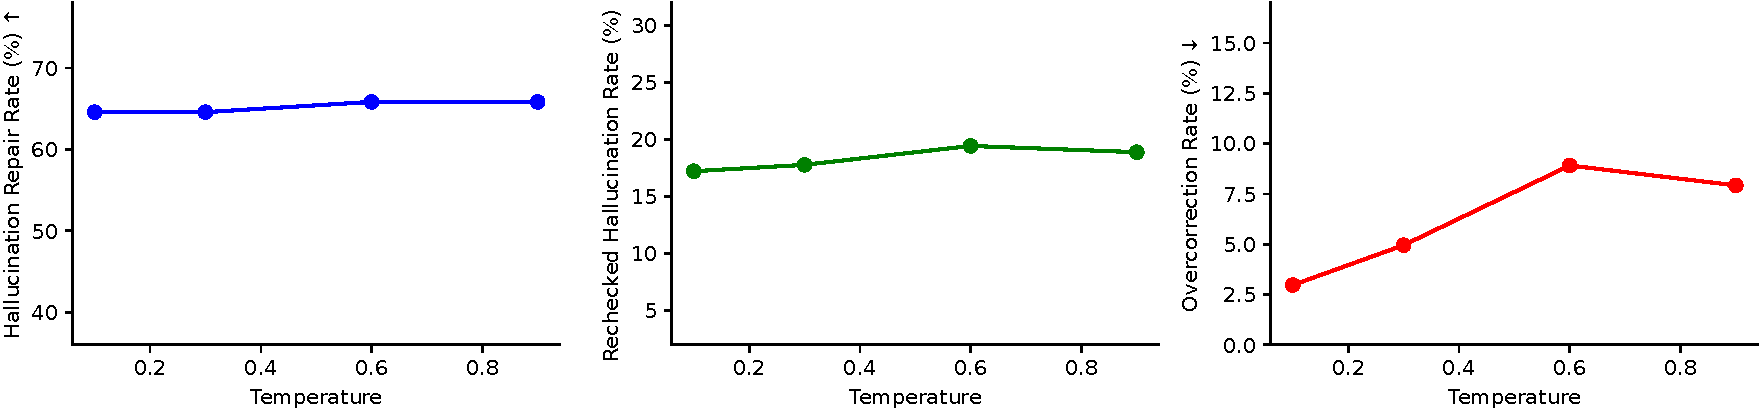
\includegraphics[width=\linewidth]{figures/rq4.1.pdf}
% %     \caption{\textbf{RQ4.1:} }
% %     \label{fig:rq4.1}
% % \end{figure}

% \subsubsection{Number of mutations}
% Although generating more mutations can potentially stabilize mutant quality and expand the repair space, thereby benefiting MutRepair’s performance, it inevitably incurs additional computational cost. To this end, we systematically evaluate MutRepair under different mutation counts. As illustrated in Figure~\ref{fig:rq4.2}, we conduct experiments on the same sampled dataset used in RQ3 and evaluate MutRepair on GPT-4o with the number of mutations set to \( N = \{0,1,3,5,7,9\} \). The results show that increasing the number of mutations yields only marginal improvements in overall repair performance. This observation explains why we adopt a moderate default setting of \(N=5\), which balances effectiveness and efficiency. We further discuss the computational overhead of MutRepair in Section \ref{sec:6.1}.


% \mybox{\textbf{Answer to RQ4: }
% Increasing the temperature does not lead to improvements of MutRepair in hallucination repair rate, while the over-correction rate increases noticeable at higher temperatures (RQ 4.1).

% Increasing the number of generated mutations does not lead to significant performance gains for MutRepair (RQ 4.2).
% }
     
% \subsection{Ablation Study (RQ5)}
% In this RQ, we conduct an ablation study to isolate the contributions of mutation-guided repair and aggregation strategies. Specifically, we compare three variants: (1) MutRepair without mutation and without aggregation, (2) MutRepair with mutation and ranking-based aggregation, and (3) pass@6, an upper-bound setting that measures the proportion of instances in which at least one correct repair is obtained among six repaired candidates generated from the base response and five mutations.

% Figure \ref{fig:rq5} shows, across all four LLMs, MutRepair with mutations consistently outperforms MutRepair without mutations. For GPT-4o, the repair rate increases from 65.15\% to 69.05\% (+3.90, +6.0\%); for GPT-5, from 49.45\% to 61.54\% (+12.09, +24.5\%); for Gemini, from 35.47\% to 46.62\% (+11.15, +31.4\%); and for Qwen3, from 40.02\% to 45.17\% (+5.15, +12.9\%). This demonstrates that mutation-guided repair combined with aggregation substantially expands the effective repair space beyond single-pass self-repair.

% The pass@6 results further reveal substantial remaining headroom. Compared to OA-RA, pass@6 increases the overall repair rate from 69.05\% to 72.76\% on GPT-4o (+3.71, +5.37\%), from 61.54\% to 65.11\% on GPT-5 (+3.57, +5.80\%), from 46.62\% to 48.81\% on Gemini (+2.19, +4.70\%), and from 45.17\% to 48.10\% on Qwen3 (+2.93, +6.49\%). These gains indicate that while aggregation already recovers a large fraction of correct repairs, there remains an approximately 5-6\% gap to the oracle upper bound, suggesting that more effective selection strategies could further close this gap.

% \mybox{\textbf{Answer to RQ5:}
% The results confirm that mutation-guided repair is a key contributor to MutRepair’s effectiveness, and that aggregation plays a critical role in identifying high-quality corrections among diverse repair candidates. However, MutRepair does not yet reach the upper bound exposed by pass@6, indicating clear headroom for improving selection strategies.
% }
     

% \subsection{Overhead Analysis}
% \begin{wraptable}{r}{7cm}
%   \centering
%   \caption{An average token\&time cost per QA-process comparison on multi models}
%   \resizebox{0.4\textwidth}{!}{
%     \begin{tabular}{c|c|c|c}
%     model & method & token cost & time cost \\
%     \midrule
%     \multirow{4}[2]{*}{gpt-4o} & CoT   & 100.61  & 4.96  \\
%           & CoVe  & 2253.68  & 22.13  \\
%           & CoVe-SE & 3623.59  & 33.61  \\
%           & MutRepair  & 4191.10  & 22.11  \\
%     \midrule
%     \multirow{4}[2]{*}{gpt-5} & CoT   & 94.58  & 12.40  \\
%           & CoVe  & 6743.49  & 114.97  \\
%           & CoVe-SE & 7320.52  & 113.26  \\
%           & MutRepair  & 3609.91  & 168.55  \\
%     \midrule
%     \multirow{4}[2]{*}{gemini} & CoT   & 95.45  & 3.68  \\
%           & CoVe  & 3620.41  & 26.88  \\
%           & CoVe-SE & 3227.44  & 24.22  \\
%           & MutRepair  & 4536.21  & 52.03  \\
%     \midrule
%     \multirow{4}[1]{*}{qwen3} & CoT   & 514.67  & 15.45  \\
%           & CoVe  & 2260.03  & 27.35  \\
%           & CoVe-SE & 3219.47  & 35.51  \\
%           & MutRepair  & 4521.08  & 21.76  \\
%     \end{tabular}
%   }
%   \label{tab:cost}
% \end{wraptable}
% Employing LLM-based pipelines that involve multiple generations and verification steps inevitably introduces additional time and token overhead, which may limit practical deployment in resource-constrained environments.

% Table~\ref{tab:cost} reports the average token consumption of MutRepair and the baselines across different models. Overall, MutRepair incurs higher token cost than single-pass baselines due to mutation generation, multi-branch repair, and aggregation. However, the overhead remains moderate when compared with strong verification-based methods such as CoVe, which also require multiple LLM calls. From a practical perspective, this trade-off is important: MutRepair demonstrates that effective hallucination repair can be achieved with manageable overhead, making it viable for real-world scenarios where both reliability and cost efficiency must be balanced.

\section{Discussion}
\subsection{Case Study}
The overall comparison of CoVe and MutRepair workflows is illustrated in Figure~\ref{fig:casestudy}. We use the hallucinated example in Figure~\ref{fig:haluexample} to illustrate how our approach repairs a case that the baseline CoVe fails to correct. Given the question “Legal tender laws in the US require all businesses to accept what for payment?”, the base response “It is illegal for a business to be cash-free in the US.” contains a hallucinated statement. CoVe first extracts verification targets from this response, including key entities and claims such as \emph{legal tender laws}, \emph{businesses}, \emph{accept cash}, and \emph{cash-free is illegal}. Based on these extracted items, CoVe formulates multiple verification questions that appear well aligned with the original query, such as: (i) \emph{What does U.S. law define as legal tender?} (ii) \emph{Do legal tender laws require businesses to accept cash?} (iii) \emph{Are cashless businesses legal in the United States?}, as well as other verification questions. CoVe then answers these verification questions using a Search Engine to obtain corresponding verification answers. Finally, CoVe feeds all verification questions and their answers into a new round of prompting to revise the initial response by aggregating the self-generated evidence. During verification, one answer states that, in some U.S. states, payment laws indicate that operating a completely cashless business is not legally permitted. As this evidence is incorporated into the revision step, CoVe produces a final answer that remains aligned with the base response and thus does not correct the hallucinated statement.

In contrast, our approach starts from the same base response but applies mutation-based transformations to systematically generate a set of response mutants that are semantically equivalent under the original assumption. These mutated responses are then independently examined by the LLM, which is prompted to re-evaluate each mutation with respect to the original question and revise them if potential factual errors or hallucinations are detected. This process yields a collection of repaired candidate answers produced from different mutated perspectives. Finally, these repaired candidates are jointly assessed via pairwise comparisons by an LLM to select the most reliable answer as the final output. In this example, our method successfully revises the base response into a corrected answer without relying on any external knowledge source and agent, precisely reflecting the fact that there is no specific law requiring all businesses in the United States to accept cash. CoVe, despite employing an external agent, fails to repair the hallucination in the base response.

\begin{figure*}[t]
    \centering
    
\includegraphics[width=1\textwidth]{figures/casestudy.pdf}
    \caption{A Case Comparison of the CoVe and MutRepair workflow on a hallucination QA example.}
    \label{fig:casestudy}
\end{figure*}


\subsection{Ethics Consideration}
Hallucination repair in open-domain question answering inevitably involves normative judgments about what constitutes ``factual correctness'', because many questions admit ambiguity due to subjectivity, incomplete evidence, or socially contested interpretations. In such cases, the line between hallucination, uncertainty, and a plausible interpretation may be unclear, and a repair method could be criticized for implicitly imposing a single notion of truth. This concern is particularly relevant when system outputs are treated as authoritative, since an overly confident “repaired” answer may crowd out legitimate uncertainty or alternative viewpoints.

MutRepair’s fault-assumption paradigm encourages the model to critically re-examine responses while preserving the original answer when no error is detected, and its mutation process exposes inconsistencies that often correlate with weak factual grounding. This pipeline therefore tends to penalize brittle, overconfident claims: candidates that remain inconsistent across mutations are less likely to be selected by the aggregation stage, which uses pairwise comparisons to identify the answer that is consistently preferable to alternatives across independently repaired candidates. In ethically sensitive or contested scenarios, this reflective and comparative design helps the model avoid unwarranted certainty and reduces the likelihood that a single spurious rationale dominates the final output. Taken together, the combination of a controlled ground-truth regime and empirically low over-correction supports the claim that ethical ambiguity does not materially affect our main conclusions in this experimental scope.

\section{Threats to Validity}
\paragraph{Internal Validity}
% Despite the strong results, our approach’s final performance still falls short of the theoretical maximum that mutation-based repair could achieve under ideal conditions. In other words, there remains a noticeable gap between our current outcomes and the upper bound where every correct repair is perfectly recognized. However, this gap does not materially undermine our findings. Even with room for improvement, the method consistently and significantly outperforms strong baselines on all benchmarks. The robust gains we observe coupled with low rates of over-correction, indicate that the core conclusions hold: our mutation-guided self-repair framework is highly effective, and the residual performance gap mainly highlights an opportunity for further refinement rather than a fundamental flaw.
Although MutRepair consistently outperforms all baselines, there remains a small gap to the pass@6 oracle upper bound, indicating that some correct repairs among the generated candidates are not always selected by the current aggregation strategy. This reflects limitations of the present LLM-as-judge implementation rather than of mutation-guided repair itself, and the gap is relatively small (about 6\%). In addition, minor implementation-level factors -- such as occasional low-diversity mutations or imperfect pairwise judgments -- may introduce noise in individual cases. However, these factors are unlikely to systematically bias results, as the same pipeline is applied uniformly across all settings. Given the large and statistically significant improvements of MutRepair, strong robustness across repeated runs, and consistently low over-correction rates, these internal threats do not materially affect our main conclusion.


\paragraph{External Validity}
A potential external threat comes from the inherent stochasticity of large language models, which can lead to variability in replication. This is particularly relevant for the Chain-of-Verification baseline, where the model dynamically extracts entities and generates follow-up verification questions. Small differences in these generated questions or the verification chain can sometimes cause the baseline’s behavior to diverge slightly from the intended scope. Nonetheless, the impact on our overall conclusions is minimal. We mitigated reproducibility concerns by using CoVe’s original codebase and default settings, ensuring any variability reflects the method’s nature rather than an implementation error. In practice, we found that the performance trends remained consistent despite LLM randomness, our approach retained its clear advantage over the baselines, indicating that stochastic variations do not compromise the validity of our comparative results.


% \subsubsection{Computational Cost Analysis}
% Beyond repair effectiveness, we further analyze the practical overhead introduced by MutRepair. Since MutRepair involves multiple generations and answer aggregation, it inevitably incurs additional time and token costs (including both input and output tokens) compared to single-pass baselines.

% Table~\ref{tab:cost} reports the average token consumption and runtime per QA process across different models. As expected, MutRepair requires more tokens than CoT due to its multi-branch repair and aggregation pipeline. Nevertheless, its token overhead consistently remains lower than that of the top baseline, which depend on explicit claim extraction, verification question generation, and multiple LLM calls with long-context prompts. This comparison suggests that mutation-guided repair can achieve competitive reliability improvements with substantially lower token costs than verification-centric pipelines. For instance, on GPT-5, MutRepair reduces the average token cost from CoVe’s 6743.49 tokens to 1804.96 tokens, corresponding to a relative reduction of 73.2\%.

% \begin{table}[htbp]
%   \centering
%   \caption{\textbf{RQ1.2:} An average token\&time cost per QA-process comparison on multi models}
%   \label{tab:cost}
%   \resizebox{0.95\columnwidth}{!}{
%       \begin{tabularx}{\linewidth}{
%         >{\centering\arraybackslash\hsize=0.6\hsize}X | 
%         >{\centering\arraybackslash\hsize=1.2\hsize}X | 
%         >{\centering\arraybackslash\hsize=1.2\hsize}X
%       }
%         \toprule
%         model & method & token cost \\
%         \midrule
%         \multirow{5}[2]{*}{gpt-4o} & CoT   & 100.61  \\
%               & CoVe  & 2253.68  \\
%               & CoVe-SE & 3623.59  \\
%               & DrHall  & 2251.93  \\
%               & \textbf{MutRepair}  & \textbf{2095.55}  \\
%         \midrule
%         \multirow{5}[2]{*}{gpt-5} & CoT   & 94.58  \\
%               & CoVe  & 6743.49  \\
%               & CoVe-SE & 7320.52  \\
%               & DrHall  & 2207.91  \\
%               & \textbf{MutRepair}  & \textbf{1804.96}  \\
%         \midrule
%         \multirow{5}[2]{*}{gemini} & CoT   & 95.45  \\
%               & CoVe  & 3620.41  \\
%               & CoVe-SE & 3227.44  \\
%               & DrHall  & 2300.74  \\
%               & \textbf{MutRepair}  & \textbf{2268.11}  \\
%         \midrule
%         \multirow{5}[1]{*}{qwen3} & CoT   & 514.67  \\
%               & CoVe  & 2260.03  \\
%               & CoVe-SE & 3219.47  \\
%               & DrHall  & 2234.46  \\
%               & \textbf{MutRepair}  & \textbf{2260.54}  \\
%         \bottomrule
%       \end{tabularx}
%   }
% \end{table}


\section{Related Work}
% LLM Hallucination Detection and Mitigation
A large body of recent work focuses on hallucination detection and mitigation, one direct line of approaches compares model-generated outputs against external or curated knowledge sources to assess factual consistency~\cite{guo2022survey, galitsky2025truth}. Another line leverages token-level signals, such as confidence scores, generation probabilities, or entropy, to estimate model uncertainty and detect hallucinated responses~\cite{varshney2023stitch}. Beyond knowledge- and signal-based methods, some studies adopt an LM-vs-LM paradigm, where an examiner model interrogates or cross-checks the outputs of an examinee model to expose inconsistencies and factual errors~\cite{cohen2023lm}. More recently, an increasing number of works explore self-detection, prompting an LLM to analyze, critique, and verify its own outputs through natural language reasoning~\cite{zhao2024knowing}.

% LLM Hallucination Repair
Beyond detection, an emerging line of research has begun to explore hallucination repair and correction, which aim to automatically transform hallucinated LLM outputs into factually reliable responses. Many existing approaches follow a similar paradigm to hallucination detection, relying on additional knowledge signals to guide the correction process. These signals may come from token-level statistics such as confidence or uncertainty estimates~\cite{vazhentsev2025token}, external knowledge bases or retrieval systems~\cite{li2025rac}, auxiliary LLM agents~\cite{kwartler2024good}, or search engines and web resources~\cite{vladika2025correcting}.

% LLM Hallucination Self-correction
Hallucination repair is closely related to the broader research topic of LLM self-correction, which investigates whether and how language models can identify and correct their own errors without external supervision~\cite{manakul2023selfcheckgpt}. Some work achieves correction by incorporating environmental feedback, such as explicit True/False signals or reward feedback~\cite{shinn2023reflexion}. However, extensive empirical studies have shown that in the complete absence of external feedback, LLMs often struggle to engage in effective self-reflection, particularly in recognizing their own reasoning errors~\cite{huang2023large}. Recent work further suggests that this limitation can be partially alleviated when models are explicitly guided toward potential error locations or failure points through targeted prompting~\cite{tyen2024llms}. Motivated by these findings, existing research on self-correction mainly follows two directions. One line of work enhances self-correction capabilities during training, for example through imitation learning or reinforcement learning, to improve error awareness and correction behaviors~\cite{kumar2025training}. Another line designs inference-time reflection and correction pipelines that prompt LLMs to examine, critique, and revise their own outputs~\cite{ayala2024reducing}. In contrast to these approaches, which primarily aim to improve or elicit general self-correction abilities, our work focuses on systematic, output-level hallucination repair after responses are generated.

% SE approaches for LLM reliability
Recent work has begun to adapt software engineering methodologies such as metamorphic testing, robustness testing, and fault analysis to systematically evaluate and diagnose LLM behaviors. For example, \cite{yang2025hallucination} leverage metamorphic relations to detect hallucinations by checking consistency violations under controlled input transformations, while \cite{wu2025detecting, li2024drowzee} adopt metamorphic testing techniques to systematically probe hallucination behaviors. Beyond detection, \cite{song2025progco} proposes a program-guided self-correction approach, where the model generates verification programs and reasons as if executing them to validate an initial answer. Through multiple rounds of verification and refinement, the LLM iteratively improves its response until it deems the output sufficiently correct. However, this method does not operate in a no external resource setting, as it relies on program execution-based verification to guide the correction process. Moreover, their work targets reasoning, selection and mathematical problem-solving tasks, rather than open-domain factual hallucination repair. These studies demonstrate that software engineering principles provide a powerful foundation for understanding, testing, and improving LLM reliability.

% Summary
Our method is distinct from prior work on hallucination detection and mitigation by explicitly focusing on hallucination repair. Under a self-contained setting, it does not rely on any external knowledge sources, in contrast to approaches that depend on retrieval, tools, or external agents. Moreover, rather than directly verifying whether an answer contains hallucinations, we assume the presence of potential faults and encourage the model to actively explore and repair them through fault-aware self-assessment. By constructing structured mutations, our approach further expands the repair space, enabling the model to more effectively expose and correct latent factual errors through systematic perturbations.


% In summary, MutRepair is positioned at the intersection of hallucination self-correction and software testing inspired reliability methods, but targets output-level repair after an LLM response is produced. Unlike many repair/correction approaches that rely on external knowledge signals (e.g., retrieval, search, or auxiliary agents) or training-time enhancement, MutRepair operates in a zero-resource setting and treats fact-conflicting generations as repairable response-level faults. It leverages mutation-guided response variants and fault-injected revision to construct a structured repair space, and then selects a final correction via comparative LLM-as-judge aggregation.


\section{Conclusions}
In this paper, we presented MutRepair, a self-contained framework for actively repairing nonfactual hallucinations in large language model outputs. Inspired by metamorphic testing and automated repair paradigms from software engineering, MutRepair systematically constructs metamorphic response mutations, triggers fault-injected self-repair, and aggregates multiple repaired candidates through LLM-as-judge strategies to select a final corrected answer. Extensive experiments on three hallucination benchmarks across four representative LLMs demonstrate that MutRepair consistently outperforms strong baselines in hallucination repair effectiveness, while maintaining lower over-correction (i.e., erroneous modification of initially correct answers). 

Beyond empirical gains, MutRepair demonstrates the practical viability of self-contained hallucination repair under realistic black-box deployment constraints. By eliminating reliance on external knowledge, auxiliary agents, or retraining pipelines, MutRepair provides a lightweight and easily deployable mechanism for improving factual reliability in existing LLM-based systems.

% There are several promising directions for future work. First, we plan to extend MutRepair with richer and more diverse mutation operators and metamorphic transformations, enabling broader coverage of semantic variations and more powerful repair space exploration. Second, we aim to apply MutRepair to more complex generation settings, including long-form generation, multi-document synthesis, and multi-turn dialogue, where hallucinations a

% Beyond improving hallucination repair performance, MutRepair highlights a broader perspective: hallucinations can be treated not only as detection targets, but as repairable faults in LLM-generated outputs. We believe this work opens new opportunities for integrating software testing and automated repair principles into the reliability engineering of LLM-based systems. Future work includes extending MutRepair to richer metamorphic relations, more complex generation settings such as long-form and multi-turn interactions, and exploring hybrid repair frameworks that incorporate external knowledge when available.

\section*{Data Availability}
\noindent\textbf{Code Repository} containing implementation code and experimental scripts is publicly available at: \url{https://anonymous.4open.science/r/LLMHalluMiti-BD85/}


\bibliographystyle{IEEEtran}
\bibliography{references}
\end{document}
\endinput
